\documentclass[10pt]{article}
\newcommand\tab[1][1cm]{\hspace*{#1}}
\usepackage{amsmath}
\usepackage{graphicx}
\newcommand{\ihat}{\boldsymbol{\hat{\textbf{\i}}}}
\newcommand{\jhat}{\boldsymbol{\hat{\textbf{\j}}}}
\graphicspath{ {./} }
\usepackage[margin=1in]{geometry}
\begin{document}

\paragraph{Nicole Pagane $|$ 05/16/19 $|$ Numerical Methods}

\section*{Final Project: Modeling Baltimore Policing}

\subsection*{Introduction}
Baltimore is the 30th largest city in the United States yet houses the 8th largest police department in the nation. Oddly enough, the Baltimore Police Department (BPD) often complains of being sorely understaffed. How can we make sense of this discrepancy, especially with regard to recent events such as Freddie Gray?\\
\\
First, we look to social theorists George Kelling and James Wilson, who---in their 1982 article on Broken Windows theory---state that increased presence of "foot patrol had not reduced crime rates". However, the residents of patrolled areas felt safer since the patrolmen mediated "the fear of being bothered by disorderly people". Thus, most major cities err on the side of too many officers/patrolmen to ensure their citizens feel that their neighborhoods are safe and in order. However, the definition of "order" when it comes to safety is thus very neighborhood-specific. For example, in a wealthy neighborhood, the  residents would think that broken windows or other signs of poverty and urban decay is not typical for their neighborhood; therefore police would monitor signs of poverty and anyone who fits to that mold in that neighborhood. Unfortunately in the US with its racial wealth gap and highly segregated urban neighborhoods, these classist prejudices are most typically manifested in a racist manner.\\
\\
This is seen through the policy implementation of Broken Windows policing---stop and frisk. Stop and frisk enables police officers to stop and check the possessions of any pedestrian if they have any reasonable suspicion that the pedestrian is harboring any dangerous contraband. Rather than needing  probable cause to act, the police are justified to use their discretion rather than the law to police citizens under stop and frisk. In NYC under the mayorship of Michael Bloomberg, stop and frisk was at its highest use; however, a federal judge ruled it unconstitutional due to the racial disparities in the stops---of all stop and frisk stops, 52\%\ were black though they make up only 23\%\ of the NYC population, and out of these 2.2 million stops of black citizens under the reign of Bloomberg, only 1\%\ led to finding dangerous contraband.\\
\\
Thus, my question is: with Baltimore's very poor recent policing of its black citizens (fun fact: the BPD is under a federal consent decree with the DOJ to drastically reform itself after a 2015 investigation found racist policing practices that violated the First, Fourth, and Fourteenth Amendments of Baltimore citizens) coupled with the fact that Michael Bloomberg is a wealthy donor who implemented a racist policing strategy that disproportionately harmed black citizens, should Johns Hopkins implement a private police force when the training, judgment, and policing strategies of the involved parties have all been found by the court to be unconstitutional and racist?\\
\\
To answer this question, I will construct a Broken Windows theory model of policing to simulate the racial arrest tactics of the BPD throughout Baltimore. Since multiple studies have found that people of all races (specifically black and white) use drugs at about the same rate, all people despite their race should be arrested for drug possession crimes at similar rates. Therefore, I will use the BPD Open Data for arrests and census data, to  assess the condition of Baltimore racial policing and then fit this to my model via MCMC.

\subsection*{Methods and Numerics}
\subsubsection{Model Paradigm}
Police patrol act to maintain "order" according to Broken Windows theory. However, Baltimore City is very segregated, so "order" maintenance has a racial connotation. Therefore, if we assume similar drug use between white and black Baltimore citizens, we can evaluate the racial bias from stop and frisk and other racial policing tactics for drug arrests of black citizens relative to white citizens in different Baltimore neighborhoods. We assume the rate of arrest for black and white citizens are the same, but the arrest rate is enhanced for citizens in a neighborhood that they are a minority in. Thus, you can expect to see over-policing of white citizens in black neighborhoods and over-policing of black citizens in white neighborhoods. The difference in over-policing rates will thus reveal a parameterized racial bias of BPD arrests.

\subsubsection{Data Curation and Visualization}
From the BPD and census, I gathered arrest and population data. Through the use of the geopandas package, I was able to read in, manipulate, and visualize spatial data. Here is the raw drug arrest data for black and white citizens in different neighborhoods.   \begin{figure}[!htb]
    \begin{minipage}{\textwidth}
     \caption{Raw Drug Arrests}
     \centering
     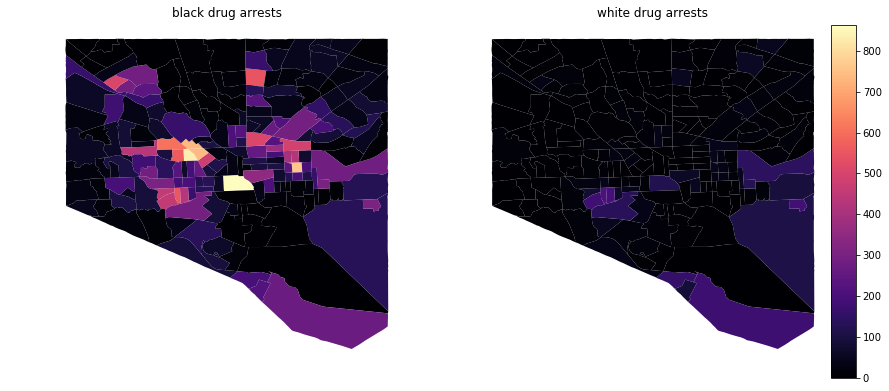
\includegraphics[width=0.6\textwidth]{rawdrug.png}
   \end{minipage}\hfill
 \end{figure}\\
 This doesn't make much sense without understanding where Baltimore citizens live. Below I show the proportions of black and white residents in each neighborhood. The typical black butterfly and white L can be seen.
   \begin{figure}[!htb]
    \begin{minipage}{\textwidth}
     \caption{Scaled Populations}
     \centering
     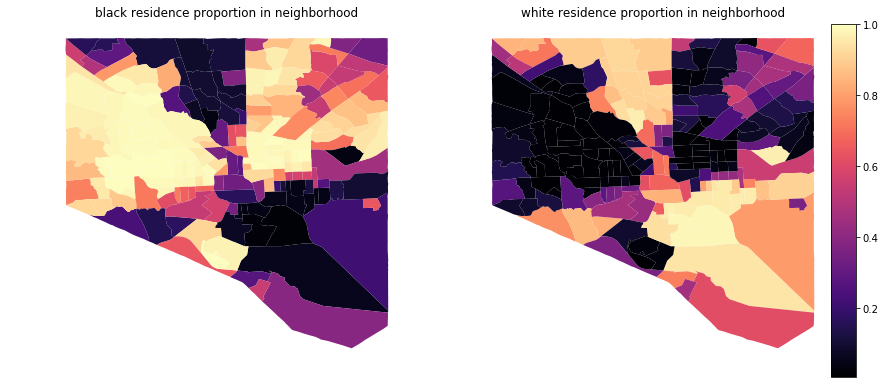
\includegraphics[width=0.6\textwidth]{scalelive.png}
   \end{minipage}\hfill
 \end{figure}\\
 Thus, we can now reconstruct drug arrests by their racial composition in each neighborhood. However, we see a spreading of the black butterfly and disappearance of the white L. 
    \begin{figure}[!htb]
    \begin{minipage}{\textwidth}
     \caption{Scaled Drug Arrests}
     \centering
     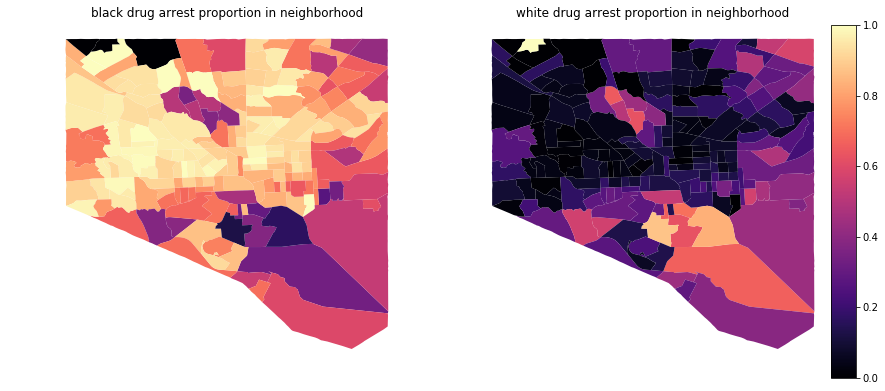
\includegraphics[width=0.6\textwidth]{scaledrug.png}
   \end{minipage}\hfill
 \end{figure}\\
This means that in white-majority neighborhoods, black citizens are being arrested more for drug crimes than they exist in the population. To better visualize this, I have reproduced a plot that shows the ratio of racial drug arrests to racial population proportions for each neighborhood (log-scaled). 
    \begin{figure}[!htb]
    \begin{minipage}{\textwidth}
     \caption{Ratio of Scaled Drug Arrests to Population}
     \centering
     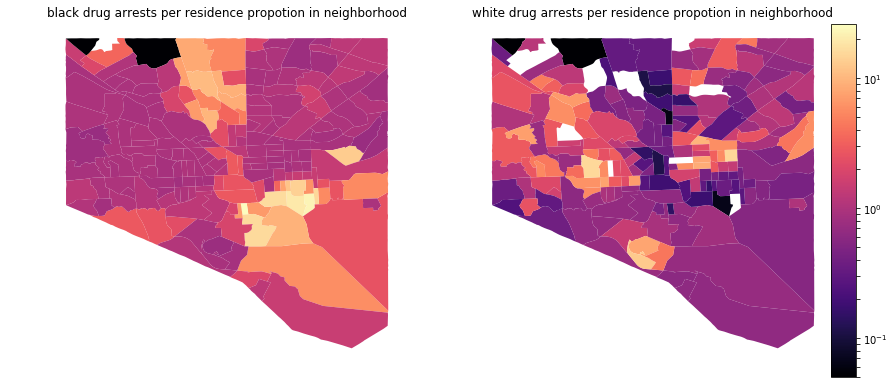
\includegraphics[width=0.6\textwidth]{logdrugpop.png}
   \end{minipage}\hfill
 \end{figure}\\
 We now see the typical segregation patterns of Baltimore in both black and white over-policing rates in neighborhoods where they are in the minority. For black citizens, we see that along the white L, they are about 10 times over-policed---i.e. the black arrest proportion for these neighborhoods are 10 times more than the black residential proportion. You see similar behavior in the white over-arrest plot but it is not as spatially resolved in black neighborhoods as it is for black over-arrest in white-majority areas. We want to parameterize this difference in over-arrest rates to determine the racial bias in Broken Windows policing.
 
 \subsubsection{Model Development}
 At first I used a kinetic Monte Carlo to simulate policing since I was dealing with rare, independent Poisson events at low integer numbers. Thus, I wanted to use a stochastic simulation over a deterministic differential equation. The rates of policing were defined as:
 \begin{equation}
a_b = r_b(p_wBW_b + p_b)p_P
\end{equation}
\begin{equation}
a_w = r_w(p_w + p_bBW_w)p_P
 \end{equation}
 where $a_b$ and $a_w$ are the observed arrest rate for black and white citizens; $r_b = r_w$ is the average rate that BPD arrests any citizen; $p_w$ and $p_b$ are the proportions of white and black citizens in each neighborhood;  $BW_b$ and $BW_w$ are the broken windows parameters that reflect the over-policing of black and white citizens in white and black-majority neighborhoods respectively; and $p_P$ is the distribution of the 2514 BPD officers around the city, stationed in accordance to violent crime statistics. I was able to use the BPD and census data to determine $r_b = r_w = 7.875$ arrests per day, $p_w$ and $p_b$ for each neighborhood, and  $p_P$ across the city.
     \begin{figure}[!htb]
    \begin{minipage}{\textwidth}
     \caption{Drug Rates}
     \centering
     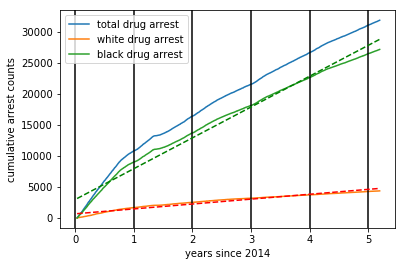
\includegraphics[width=0.465\textwidth]{drugrates.png}
   \end{minipage}\hfill
 \end{figure}\\
 Above, shows the BPD arrest data using linear regression to obtain the black and white arrest rates of 13.59 per day and 2.15 per day, respectively. Thus, we will use the average of these trends. \\
 \\
 In the kinetic Monte Carlo, each time-step allowed for one drug arrest in one neighborhood, and this neighborhood was sampled in accordance with officer density---which is then connected to violent crime locations. With profiling, I soon realized that a kinetic Monte Carlo was way too slow to do appreciable fitting with, so I instead resorted back to a linearized ODE as seen by the above differentials. Below shows how the comparison of the average of 40 kinetic Monte Carlos with the parameters, $r_b = r_w = 7.875$ per day, $BW_b = 5.5$, and $BW_w = 0.1$ with the quicker linearized ODE.
 \begin{figure}[!htb]
 \begin{minipage}{0.5\textwidth}
     \caption{Average of 40 Kinetic Monte Carlos}
     \centering
     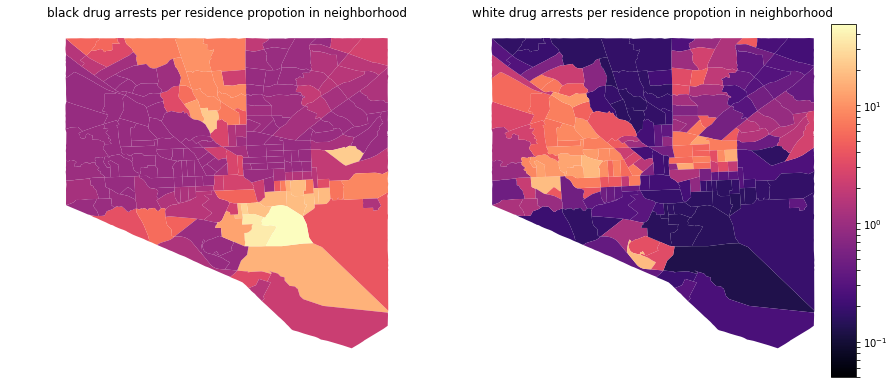
\includegraphics[width=\textwidth]{km.png}
   \end{minipage}\hfill
   \begin{minipage}{0.5\textwidth}
     \caption{Linearized ODE Solution}
     \centering
     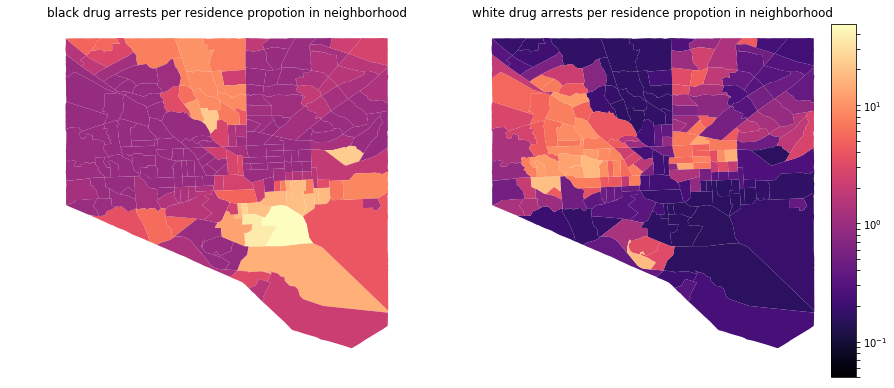
\includegraphics[width=\textwidth]{rk.png}
   \end{minipage}\hfill
 \end{figure}
 
    \begin{figure}[!htb]
    \begin{minipage}{\textwidth}
     \caption{Converging Simulation Approaches}
     \centering
     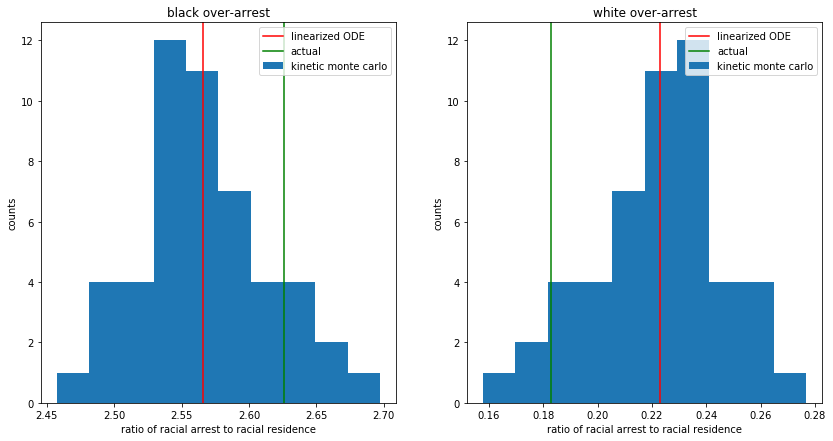
\includegraphics[width=0.6\textwidth]{kmandrk.png}
   \end{minipage}\hfill
 \end{figure}
 
 However, it is evident that the converging simulations are not reflecting the actual data, seen by the green vertical line. Thus, we turn to data fitting.
 
\subsubsection{Data fitting}
  At first, I wished to fit the model Broken Windows parameters to the data via Bayesian inference and MCMC. However, the data I am using is accumulated time-series data. Instead of having individual random variables take up different states, I have spatial data that results in only one datum per neighborhood (i.e. the number of drug arrests over a 5 year period). Thus, the construction of a likelihood function did not seem intuitive or at least in an analytic form. Thus, rather than maximizing the likelihood in a Bayesian interpretation to sample parameters in the MCMC, I try to minimize the least squared residuals (LSR) between the simulated data and the BPD data and then relate that in a pseudo Metroplis-Hastings fashion via:
  \begin{equation}
  p_{acc} = \exp{[-\frac{LSR(\theta_0) - LSR(\theta)}{0.5LSR(\theta)}]}
  \end{equation}
  where the value inside the exponential is akin to a percent deviation for the proposed parameters $\theta_0$ from the current parameters $\theta$. \\
  \\
  The proposal distributions were Gaussians with standard deviation 7.04 ($BW_b$) and 0.316 ($BW_w$). The MCMC was run for 200,000 iterations and the profiling showed that it took about 10 minutes on average to run. The parameters $BW_b$ and $BW_w$ were rotated every other iteration to try to sample the full span of the parameter spaces. The first half of the chain was thrown out as burn-in. The following plots offer a summary of the analysis:
   \begin{figure}[!htb]
 \begin{minipage}{0.5\textwidth}
     \caption{Markov chain for parameter sampling}
     \centering
     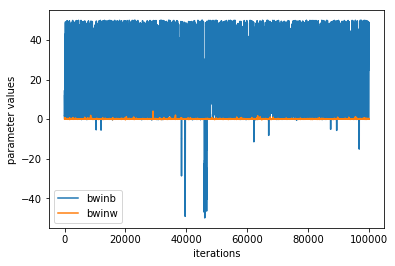
\includegraphics[width=\textwidth]{mcmciter.png}
   \end{minipage}\hfill
   \begin{minipage}{0.5\textwidth}
     \caption{Least Squared Residuals}
     \centering
     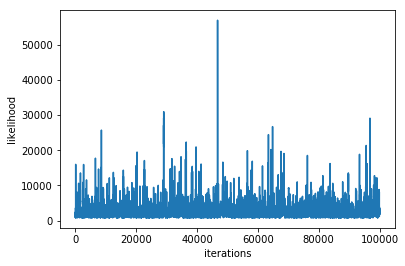
\includegraphics[width=\textwidth]{mcmclike.png}
   \end{minipage}\hfill
 \end{figure}
 
Notice how sharp deviation from the preferred range results in a sharp increase in the LSR at that iteration step. The reconstructed parameters with their spreads are shown below. 
\begin{center}
\begin{tabular}{ |c||c|c|c|c|}
 \hline
 \multicolumn{5}{|c|}{MCMC Report} \\
 \hline
  parameter & acceptance rate & 16th percentile & 50th percentile & 84th percentile \\
  \hline
 \hline
 $BW_b$ & 0.35 & 2.03 & 18.32 & 40.09\\
 \hline
 $BW_w$ & 0.10 & 0.0132 & 0.0535 & 0.1044\\
 \hline
\end{tabular}
\end{center}
The following plot reconstructs the linearized ODE simulation of BPD policing compared to the real BPD data for the metric that compares racial arrest to residential proportion.
 \begin{figure}[!htb]
 \begin{minipage}{0.5\textwidth}
     \caption{Simulation with Fit Parameters}
     \centering
     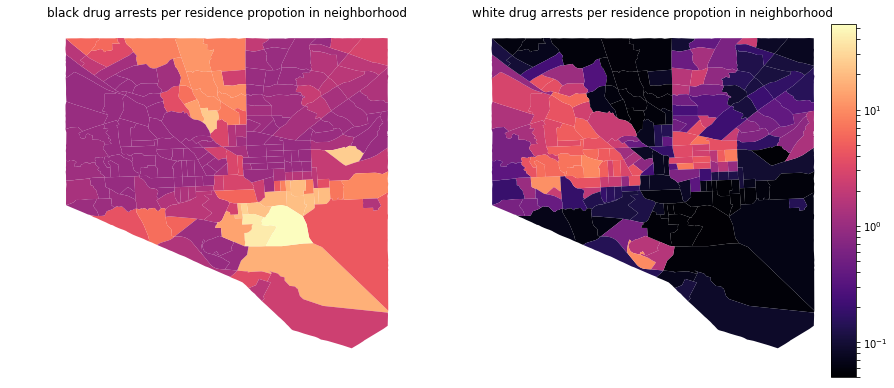
\includegraphics[width=\textwidth]{mcmcmap.png}
   \end{minipage}\hfill
   \begin{minipage}{0.5\textwidth}
     \caption{Real BDP Data}
     \centering
     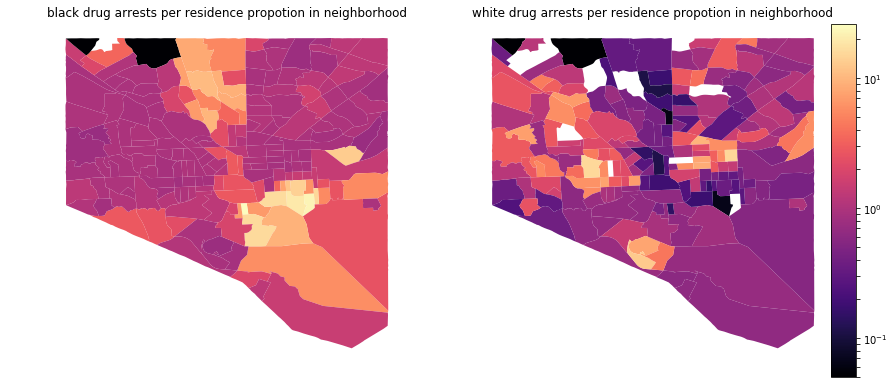
\includegraphics[width=\textwidth]{logdrugpop.png}
   \end{minipage}\hfill
 \end{figure}
 
\subsection*{Conclusion}
 Through the above analysis, we see that BPD over-polices black citizens up to 18 times for drug crimes in predominantly white neighborhoods while white citizens are typically under-policed in black neighborhoods. This brings into question once again whether a private police force should be created in a white majority neighborhood, where the officers are recruited from poorly trained BPD officers with Bloomberg-inspired policing tactics such as stop and frisk. \\
 \\
 As a complete side-note, the above analysis was supported through version control via GitHub, documentation, and profiling.

 \end{document}